\documentclass{boi2014-et}

\usepackage{enumitem}

\renewcommand{\DayNum}{2}
\renewcommand{\TaskCode}{portals}
\renewcommand{\TaskName}{Portaalid}
\renewcommand{\TaskVersion}{1.1}

\newcommand{\constant}[1]{{\tt #1}}

\begin{document}

    \begin{wrapfigure}[4]{r}{4cm}
        \vspace{-24pt}
        \includegraphics[width=4cm]{\TaskCode.jpeg}
    \end{wrapfigure}

    Labürinti on peidetud kook, mille sa tahad ära süüa.
    Sul on labürindi kaart, mis on $R$ rea ja $C$ veeruga ruudustik.
    Ruudustiku igas lahtris on üks järgmistest märkidest:
    \begin{description}[itemindent=1pt]
        \item[\constant{\#}] (ruut) tähistab seinablokki,
        \item[\constant{.}] (punkt) tähistab tühja ruutu,
        \item[\constant{S}] (suur s) tähistab sinu algasukohta,
        \item[\constant{C}] (suur c) tähistab koogi asukohta.
    \end{description}

    Sa võid kõndida ainult mööda tühje ruute ning liikuda ühelt ruudult teisele,
    kui neil on ühine külg. Lisaks on kaardil kujutatud ristkülikukujuline ala
    väljastpoolt ümbritsetud samasuguste seinablokkidega.

    Et kiiremini koogini jõuda, on sul Aperture Science\texttrademark{}
    portaaliheitepüss, mis töötab järgmiselt:
    Igal hetkel saab sellega tulistada kas
    \emph{üles}, \emph{vasakule}, \emph{alla} või \emph{paremale}.
    Kui portaal mingis suunas tulistatakse, lendab see selles suunas, kuni tabab seinablokki.
    Kui see juhtub, tekib vastava seinabloki sinupoolsele küljele portaal.

    Korraga saab eksisteerida kuni kaks portaali. Kui kaks portaali on juba olemas,
    siis portaalipüssi uuesti kasutades üks neist (sina otsustad, kumb) kaob.
    Olemasoleva portaali pihta tulistamine asendab selle portaali uuega
    (iga seinabloki ühel küljel saab korraga olla ainult üks portaal).
    Seinabloki erinevatel külgedel võivad portaalid korraga olla.

    Kui labürindis on kaks portaali, saab neid kasutada enda teleporteerimiseks.
    Seistes ühe portaali kõrval, saab sellesse sisse kõndida ning väljuda ruudul,
    mis on teise portaali kõrval. See võtab sama palju aega kui ühelt naaberruudult teisele kõndimine.

    Võib eeldada, et portaalide tulistamine ei võta aega ning ühelt ruudult teisele liikumine
    (või läbi portaalide teleporteerumine) võtab ühe ühiku aega.

    \Task

    Labürindi kaardi, oma esialgse asukoha ning koogi asukoha põhjal leida
    minimaalne koogini jõudmiseks vajalik aeg.

    \Input

    Sisendi esimesel real on kaks täisarvu: kaardi ridade arv
    $R$ ning veergude arvu $C$. Järgmised $R$ rida kirjeldavad
    kaarti. Igal real on $C$ märki: \constant{\#},
    \constant{.}, \constant{S} või \constant{C} (kirjeldatud eespool).

    Märgid \constant{S} ja \constant{C} esinevad kaardil kumbki täpselt ühe korra.

    \Output

    Väljund peab koosnema ühest täisarvust --- minimaalne aeg,
    mis on vajalik algasukohast koogini jõudmiseks.

    Võib eeldada, et algasukohast saab alati koogini jõuda.

    \Example

    \example
    {
        4 4\newline
        .\#.C\newline
        .\#.\#\newline
        ....\newline
        S...
    }
    {
        4
    }
    {
        Üks võimalik lühim käikude järjekord on: 1) liigu paremale, 2) liigu paremale,
        tulista üks portaal üles ja teine alla, 3) liigu läbi
        alumise portaali (jõuad asukohta $rida = 0,
        veerg = 2$), 4) liigu paremale ja jõuad koogini.

        \begin{center}
            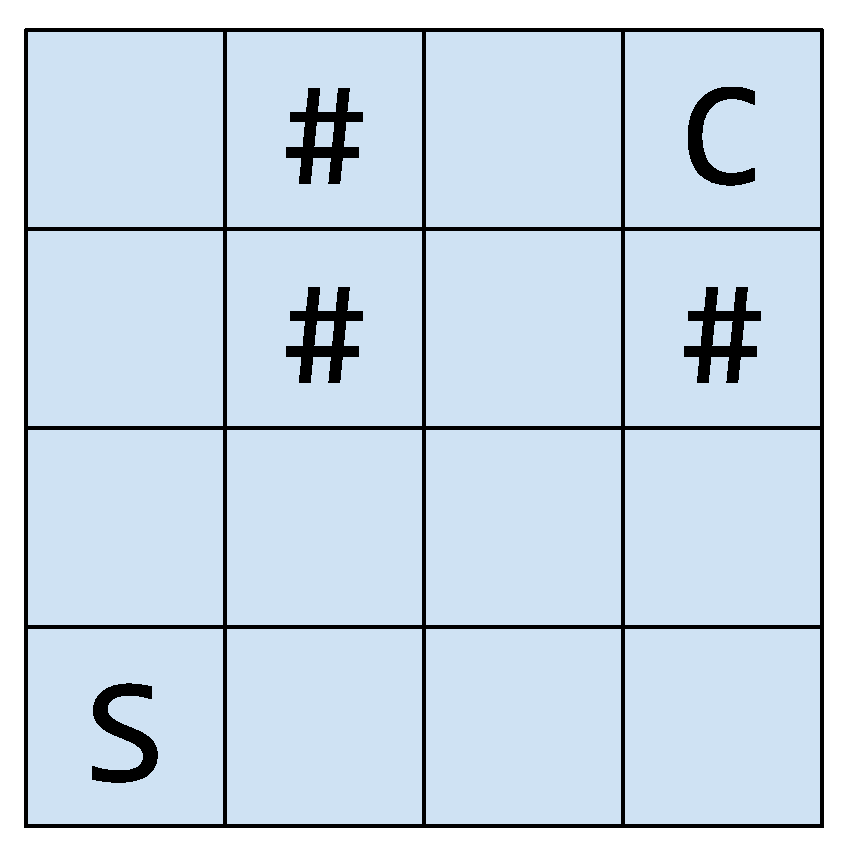
\includegraphics[width=4cm]{portals-example}
        \end{center}
    }

    \Scoring

    \begin{description}[leftmargin=0pt]
        \item[Alamülesanne 1 (11 punkti):] $1 \le R \le 10$, $1 \le C \le 10$.
        \item[Alamülesanne 2 (20 punkti):] $1 \le R \le 50$, $1 \le C \le 50$.
        \item[Alamülesanne 3 (20 punkti):] $1 \le R \le 200$, $1 \le C \le 200$.
            Iga tühja ruudu kõrval on vähemalt üks seinablokk.
        \item[Alamülesanne 4 (19 punkti):] $1 \le R \le 200$, $1 \le C \le 200$.
        \item[Alamülesanne 5 (30 punkti):] $1 \le R \le 1\,000$, $1 \le C \le 1\,000$.
    \end{description}

    \Constraints

    \begin{description}
        \item[Ajapiirang:] 1 s.
        \item[Mälupiirang:] 256 MB.
    \end{description}

\end{document}
